\documentclass[a4paper]{article}

\usepackage{inputenc}
\usepackage[british,UKenglish]{babel}
\usepackage{amsmath}
%\usepackage{titlesec}
\usepackage{color}
\usepackage{graphicx}
\usepackage{fancyref}
\usepackage{hyperref}
\usepackage{float}
\usepackage{scrextend}
\usepackage{setspace}
\usepackage{xargs}
\usepackage{multicol}
\usepackage{nameref}

\usepackage{sectsty}
\usepackage{multicol}
\usepackage{multirow}
\usepackage[procnames]{listings}
\usepackage{appendix}

\newcommand\tab[1][1cm]{\hspace*{#1}}
\hypersetup{colorlinks=true, linkcolor=black}
\interfootnotelinepenalty=10000

\newcommand{\cleancode}[1]{\begin{addmargin}[3em]{3em}\texttt{\textcolor{cleanOrange}{#1}}\end{addmargin}}
\newcommand{\cleanstyle}[1]{\text{\textcolor{cleanOrange}{\texttt{#1}}}}


\usepackage[colorinlistoftodos,prependcaption,textsize=footnotesize]{todonotes}
\newcommandx{\commred}[2][1=]{\textcolor{Red}
{\todo[linecolor=red,backgroundcolor=red!25,bordercolor=red,#1]{#2}}}
\newcommandx{\commblue}[2][1=]{\textcolor{Blue}
{\todo[linecolor=blue,backgroundcolor=blue!25,bordercolor=blue,#1]{#2}}}
\newcommandx{\commgreen}[2][1=]{\textcolor{OliveGreen}{\todo[linecolor=OliveGreen,backgroundcolor=OliveGreen!25,bordercolor=OliveGreen,#1]{#2}}}
\newcommandx{\commpurp}[2][1=]{\textcolor{Plum}{\todo[linecolor=Plum,backgroundcolor=Plum!25,bordercolor=Plum,#1]{#2}}}

\def\code#1{{\tt #1}}

\def\note#1{\noindent{\bf [Note: #1]}}

\makeatletter
%% The "\@seccntformat" command is an auxiliary command
%% (see pp. 26f. of 'The LaTeX Companion,' 2nd. ed.)
\def\@seccntformat#1{\@ifundefined{#1@cntformat}%
   {\csname the#1\endcsname\quad}  % default
   {\csname #1@cntformat\endcsname}% enable individual control
}
\let\oldappendix\appendix %% save current definition of \appendix
\renewcommand\appendix{%
    \oldappendix
    \newcommand{\section@cntformat}{\appendixname~\thesection\quad}
}
\makeatother


% "define" Scala
\usepackage[T1]{fontenc}  
\usepackage[scaled=0.82]{beramono}  
\usepackage{microtype} 

\sbox0{\small\ttfamily A}
\edef\mybasewidth{\the\wd0 }

\lstdefinelanguage{scala}{
  morekeywords={abstract,case,catch,class,def,%
    do,else,extends,false,final,finally,%
    for,if,implicit,import,match,mixin,%
    new,null,object,override,package,%
    private,protected,requires,return,sealed,%
    super,this,throw,trait,true,try,%
    type,val,var,while,with,yield},
  sensitive=true,
  morecomment=[l]{//},
  morecomment=[n]{/*}{*/},
  morestring=[b]",
  morestring=[b]',
  morestring=[b]"""
}

\usepackage{color}
\definecolor{dkgreen}{rgb}{0,0.6,0}
\definecolor{gray}{rgb}{0.5,0.5,0.5}
\definecolor{mauve}{rgb}{0.58,0,0.82}

% Default settings for code listings
\lstset{frame=tb,
  language=scala,
  aboveskip=3mm,
  belowskip=3mm,
  showstringspaces=false,
  columns=fixed, % basewidth=\mybasewidth,
  basicstyle={\small\ttfamily},
  numbers=none,
  numberstyle=\footnotesize\color{gray},
  % identifierstyle=\color{red},
  keywordstyle=\color{blue},
  commentstyle=\color{dkgreen},
  stringstyle=\color{mauve},
  frame=single,
  breaklines=true,
  breakatwhitespace=true,
  procnamekeys={def, val, var, class, trait, object, extends},
  procnamestyle=\ttfamily\color{red},
  tabsize=2
}

\lstnewenvironment{scala}[1][]
{\lstset{language=scala,#1}}
{}
\lstnewenvironment{cpp}[1][]
{\lstset{language=C++,#1}}
{}
\lstnewenvironment{bash}[1][]
{\lstset{language=bash,#1}}
{}
\lstnewenvironment{verilog}[1][]
{\lstset{language=verilog,#1}}
{}



%代码段设置
\lstset{numbers=left,
basicstyle=\tiny,
numberstyle=\tiny,
keywordstyle=\color{blue!70},
commentstyle=\color{red!50!green!50!blue!50},
frame=single, rulesepcolor=\color{red!20!green!20!blue!20},
escapeinside=``
}

\graphicspath{ {images/} }
\usepackage{float}
\usepackage{ctex}
\usepackage{graphicx}
\usepackage{color,framed}%文本框
\usepackage{listings}
\usepackage{caption}
\usepackage{amssymb}
\usepackage{enumerate}
\usepackage{xcolor}
\usepackage{bm} 
\usepackage{lastpage}%获得总页数
\usepackage{fancyhdr}
\usepackage{tabularx}  
\usepackage{geometry}
\usepackage{minted}
\usepackage{graphics}
\usepackage{subfigure}
\usepackage{float}
\usepackage{pdfpages}
\usepackage{pgfplots}
\pgfplotsset{width=10cm,compat=1.9}
\usepackage{multirow}
\usepackage{footnote}
\usepackage{booktabs}

%-----------------------伪代码------------------
\usepackage{algorithm}  
\usepackage{algorithmicx}  
\usepackage{algpseudocode}  
\floatname{algorithm}{Algorithm}  
\renewcommand{\algorithmicrequire}{\textbf{Input:}}  
\renewcommand{\algorithmicensure}{\textbf{Output:}} 
\usepackage{lipsum}  
\makeatletter
\newenvironment{breakablealgorithm}
  {% \begin{breakablealgorithm}
  \begin{center}
     \refstepcounter{algorithm}% New algorithm
     \hrule height.8pt depth0pt \kern2pt% \@fs@pre for \@fs@ruled
     \renewcommand{\caption}[2][\relax]{% Make a new \caption
      {\raggedright\textbf{\ALG@name~\thealgorithm} ##2\par}%
      \ifx\relax##1\relax % #1 is \relax
         \addcontentsline{loa}{algorithm}{\protect\numberline{\thealgorithm}##2}%
      \else % #1 is not \relax
         \addcontentsline{loa}{algorithm}{\protect\numberline{\thealgorithm}##1}%
      \fi
      \kern2pt\hrule\kern2pt
     }
  }{% \end{breakablealgorithm}
     \kern2pt\hrule\relax% \@fs@post for \@fs@ruled
  \end{center}
  }
\makeatother
%------------------------代码-------------------
\usepackage{xcolor} 
\usepackage{listings} 
\lstset{ 
breaklines,%自动换行
basicstyle=\small,
escapeinside=``,
keywordstyle=\color{ blue!70} \bfseries,
commentstyle=\color{red!50!green!50!blue!50},% 
stringstyle=\ttfamily,% 
extendedchars=false,% 
linewidth=\textwidth,% 
numbers=left,% 
numberstyle=\tiny \color{blue!50},% 
frame=trbl% 
rulesepcolor= \color{ red!20!green!20!blue!20} 
}

%-------------------------页面边距--------------
\geometry{a4paper,left=2.3cm,right=2.3cm,top=2.7cm,bottom=2.7cm}
%-------------------------页眉页脚--------------
\usepackage{fancyhdr}
\pagestyle{fancy}
\lhead{\kaishu \leftmark}
% \chead{}
\rhead{\kaishu 并行程序设计实验报告}%加粗\bfseries 
\lfoot{}
\cfoot{\thepage}
\rfoot{}
\renewcommand{\headrulewidth}{0.1pt}  
\renewcommand{\footrulewidth}{0pt}%去掉横线
\newcommand{\HRule}{\rule{\linewidth}{0.5mm}}%标题横线
\newcommand{\HRulegrossa}{\rule{\linewidth}{1.2mm}}
\setlength{\textfloatsep}{10mm}%设置图片的前后间距
%--------------------文档内容--------------------

\begin{document}
\renewcommand{\contentsname}{目\ 录}
\renewcommand{\appendixname}{附录}
\renewcommand{\appendixpagename}{附录}
\renewcommand{\refname}{参考文献} 
\renewcommand{\figurename}{图}
\renewcommand{\tablename}{表}
\renewcommand{\today}{\number\year 年 \number\month 月 \number\day 日}

%-------------------------封面----------------
\begin{titlepage}
    \begin{center}
    
\includegraphics[width=0.8\textwidth]{NKU.png}\\[1cm]
    \vspace{20mm}
		\textbf{\huge\textbf{\kaishu{计算机学院}}}\\[0.5cm]
		\textbf{\huge{\kaishu{并行程序设计实验报告}}}\\[2.3cm]
		\textbf{\Huge\textbf{\kaishu{SIMD加速的高斯消去算法}}}

		\vspace{\fill}
    
    % \textbf{\Large \textbf{并行程序设计期末实验报告}}\\[0.8cm]
    % \HRule \\[0.9cm]
    % \HRule \\[2.0cm]
    \centering
    \textsc{\LARGE \kaishu{姓名\ :\ 熊宇轩}}\\[0.5cm]
    \textsc{\LARGE \kaishu{学号\ :\ 2010056}}\\[0.5cm]
    \textsc{\LARGE \kaishu{专业\ :\ 计算机科学与技术}}\\[0.5cm]
    
    \vfill
    {\Large \today}
    \end{center}
\end{titlepage}

\renewcommand {\thefigure}{\thesection{}.\arabic{figure}}%图片按章标号
\renewcommand{\figurename}{图}
\renewcommand{\contentsname}{目录}  
\cfoot{\thepage\ of \pageref{LastPage}}%当前页 of 总页数


% 生成目录
\clearpage
\tableofcontents
\newpage

%--------------------------Title--------------------------------

\section{实验目标}

\begin{enumerate}
  \item 编写代码实现普通高斯消去算法以及消元子模式的高斯消去算法,并通过intrinsic方式利用X86和ARM平台上NEON、SSE、AVX、AVX512等指令集实现SIMD加速。
  \item 编写测试脚本,通过运行计时的方式,测试不同规模下不同加速算法的加速比。
  \item 利用perf等工具对实验结果进行分析,找出性能差异的原因。
\end{enumerate}

\section{核心代码}
\subsection{普通高斯消去算法}
\subsubsection{串行算法}
串行算法的实现比较简单,代码如下:
\begin{minted}[mathescape,
               linenos,
               numbersep=5pt,
               gobble=2,
               frame=lines,
               framesep=2mm,
               highlightcolor=green!40]{c}

    #define N 1024
    #define ele_t float
    
    void LU(ele_t mat[N][N], int n)
    {
        memcpy(new_mat, mat, sizeof(ele_t) * N * N); // 复制矩阵
    
        for (int i = 0; i < n; i++) // 遍历行
            for (int j = i + 1; j < n; j++)
            { //遍历列
                if (new_mat[i][i] == 0) // 当前元素已经为0,不需要消去
                    continue;
                ele_t div = new_mat[j][i] / new_mat[i][i]; // 一次性计算除数
                for (int k = i; k < n; k++)
                    new_mat[j][k] -= new_mat[i][k] * div;
            }
        // 省略:用于输出矩阵验证正确性的代码
    }
\end{minted}

\subsubsection{NEON/SSE加速}
NEON的加速实现也较为简单。不过,在实现NEON加速的过程中,作者发现了一个英特尔提供的,可以将NEON代码迁移至SSE加速的头文件。\cite{intel/arm_neon_2_x86_sse_2022}虽然对于此次作业来说,这个工具减少的代码量微乎其微,但这极大方便了程序的调试。

之所以能通过一个简单的头文件在X86平台上运行ARM NEON的代码,主要是因为SSE和NEON指令集寄存器位数都是128,且功能十分相似。NEON和SSE相较于AVX和AVX512等指令集,使用intrinsic编程的方式也十分相似,虽然寄存器位数不同,但也只需要修改调用的函数和每次load/store的数据个数即可。

此外,在研究该头文件实现时,作者发现其中的融合乘加函数其实是将一条融合乘加指令拆成两条指令实现的。然而,SSE指令集原生是支持融合乘加的,我们可以借此机会,研究融合乘加和非融合乘加SIMD对加速的影响。

关于对齐的问题,由于串行算法在实现矩阵的第j行减去第i行时,省略了第i列前的元素(在第i行i列前的元素已经全是0了),因此根据串行算法修改的来的SIMD算法“自然地”是不对齐的,通过将省略元素从i列前改为i / 4 * 4前,我们可以实现对齐的算法。

\begin{minted}[mathescape,
               linenos,
               numbersep=5pt,
               gobble=2,
               frame=lines,
               framesep=2mm,
               highlightcolor=green!40]{c}

    #ifdef __ARM_NEON
    #include <arm_neon.h>
    #endif
    
    #ifdef __amd64__
    #include <immintrin.h>
    #include "NEON_2_SSE.h" // Intel提供的用于将NEON代码迁移至SSE的头文件
    #endif
    
    #define ele_t float
    ele_t new_mat[N][N] __attribute__((aligned(64))); // 对齐
    ele_t mat[N][N];
    
    void LU_simd(ele_t mat[N][N], int n)
    {
        memcpy(new_mat, mat, sizeof(ele_t) * N * N); // 复制矩阵
    
        for (int i = 0; i < n; i++) // 遍历行
            for (int j = i + 1; j < n; j++)
            {                           //遍历列
                if (new_mat[i][i] == 0) // 当前元素已经为0,不需要消去
                    continue;
                ele_t div = new_mat[j][i] / new_mat[i][i];
                float32x4_t mat_j, mat_i, div4 = vmovq_n_f32(div);
    #ifdef ALIGN // 是否对齐
                for (int k = i / 4 * 4; k < n; k += 4)
    #else
                for (int k = i; k < n; k += 4)
    #endif
                {
                    mat_j = vld1q_f32(new_mat[j] + k);
                    mat_i = vld1q_f32(new_mat[i] + k);
    #ifdef USE_FMA // 使用融合乘加
                    vst1q_f32(new_mat[j] + k, _mm_fnmadd_ps(mat_i, div4, mat_j));
    #else
                    vst1q_f32(new_mat[j] + k, vmlsq_f32(mat_j, div4, mat_i));
    #endif
                }
            }
    }
\end{minted}

\subsubsection{AVX加速}
AVX加速和NEON/SSE加速的编程极为相似,仅仅是在函数命名和参数上有微小区别。不过需要注意的是AVX的对齐和不对齐load/store使用的是不同的函数。

AVX512的实现与AVX高度相似,这里不再赘述。

\begin{minted}[mathescape,
               linenos,
               numbersep=5pt,
               gobble=2,
               frame=lines,
               framesep=2mm,
               highlightcolor=green!40]{c}

        for (int i = 0; i < n; i++)
            for (int j = i + 1; j < n; j++)
            {
                if (new_mat[i][i] == 0)
                    continue;
                ele_t div = new_mat[j][i] / new_mat[i][i];
                __m256 mat_i, mat_j, div8 = _mm256_set1_ps(div);
    #ifdef ALIGN
                for (int k = i / 8 * 8; k < n; k += 8)
    #else
                for (int k = i; k < n; k += 8)
    #endif
                {
    #ifdef ALIGN
                mat_j = _mm256_load_ps(new_mat[j] + k);
                mat_i = _mm256_load_ps(new_mat[i] + k);
                _mm256_store_ps(new_mat[j] + k, _mm256_fnmadd_ps(mat_i, div8, mat_j));
    #else
                mat_j = _mm256_loadu_ps(new_mat[j] + k);
                mat_i = _mm256_loadu_ps(new_mat[i] + k);
                _mm256_storeu_ps(new_mat[j] + k, _mm256_fnmadd_ps(mat_i, div8, mat_j));
    #endif  
                }
            }
\end{minted}

\subsection{消元子模式的高斯消去算法}
\subsubsection{数据结构相关代码}
在消元子模式的高斯消去算法中,消元子和被消元行矩阵采用位图方式存储,由于实验中使用的数据集的矩阵列数大多不是4、8、16的整倍数,这给我们提供了实验对齐和不对齐性能差距的机会。因此作者设置了两行可以通过宏定义激活的代码,它将增加矩阵的行数到16的整倍数。

此外,由于数据集采用的是稀疏矩阵,而程序内部运算是位图格式,因此还需要设计读入和转换的代码。需要注意的是,为了方便消元子的查找以及将被消元子升格为消元子的操作,消元子矩阵被定义为了正方形矩阵。

\begin{minted}[mathescape,
               linenos,
               numbersep=5pt,
               gobble=2,
               frame=lines,
               framesep=2mm,
               highlightcolor=green!40]{c}

    #ifndef DATA
    #define DATA "./Groebner/6_3799_2759_1953/"
    #define COL 3799
    #define ELE 2759
    #define ROW 1953
    #endif
    
    #define mat_t unsigned int
    #define mat_L 32
    
    mat_t ele[COL][COL / mat_L + 1] = {0};
    mat_t row[ROW][COL / mat_L + 1] = {0};
    
    #ifndef ALIGN
    mat_t ele_tmp[COL][COL / mat_L + 1] = {0}; // 消元子矩阵为正方形
    mat_t row_tmp[ROW][COL / mat_L + 1] = {0};
    #else
    mat_t ele_tmp[COL][(COL / mat_L + 1) / 16 * 16 + 16] __attribute__((aligned(64))) = {0};
    mat_t row_tmp[ROW][(COL / mat_L + 1) / 16 * 16 + 16] __attribute__((aligned(64))) = {0};
    #endif
    
    int main()
    {
        // 读取数据集-消元子
        ifstream data_ele((string)DATA + (string) "1.txt", ios::in);
        int temp, header;
        string line;
        for (int i = 0; i < ELE; i++)
        {
            getline(data_ele, line);
            istringstream line_iss(line);
            line_iss >> header; // 先确定读入消元子的首元素
            ele[header][header / mat_L] += (mat_t)1 << (header % mat_L);
            // 将这一行消元子存进首元素对应的行,保证消元子矩阵为上三角形态,保证对角线的对应关系
            while (line_iss >> temp)
                ele[header][temp / mat_L] += (mat_t)1 << (temp % mat_L);
        }
        data_ele.close();
    }
\end{minted}

\subsubsection{串行算法}
串行算法实现比较简单,代码如下:

\begin{minted}[mathescape,
               linenos,
               numbersep=5pt,
               gobble=2,
               frame=lines,
               framesep=2mm,
               highlightcolor=green!40]{c}

    void groebner(mat_t ele[COL][COL / mat_L + 1], mat_t row[ROW][COL / mat_L + 1])
    {
        // ele=消元子,row=被消元行
        memcpy(ele_tmp, ele, sizeof(mat_t) * COL * (COL / mat_L + 1));
        memcpy(row_tmp, row, sizeof(mat_t) * ROW * (COL / mat_L + 1));
        for (int i = 0; i < ROW; i++)
        { // 遍历行
            for (int j = COL; j >= 0; j--)
            { // 遍历列
                if (row_tmp[i][j / mat_L] & ((mat_t)1 << (j % mat_L)))
                { // 当前元素有值,需要进行处理
                    if (ele_tmp[j][j / mat_L] & ((mat_t)1 << (j % mat_L)))
                    { // 有对应消元子,对当前行进行异或
                        for (int p = COL / mat_L; p >= 0; p--)
                            row_tmp[i][p] ^= ele_tmp[j][p];
                    }
                    else
                    { // 没有对应消元子,对当前行进行升格
                        memcpy(ele_tmp[j], row_tmp[i], (COL / mat_L + 1) * sizeof(mat_t));
                        break;
                    }
                }
            }
        }
        // 省略:以稀疏矩阵格式输出row_tmp,已与数据集中的参考结果对比一致
    }
\end{minted}

\subsubsection{NEON/SSE加速}
NEON/SSE的加速实现比较简单,为了方便处理,对于需要异或每一行的前面可以被寄存器宽度整除的元素进行SIMD加速运算,最后剩下来的几个元素则正常串行异或。

\begin{minted}[mathescape,
               linenos,
               numbersep=5pt,
               gobble=2,
               frame=lines,
               framesep=2mm,
               highlightcolor=green!40]{c}

    void groebner_simd(mat_t ele[COL][COL / mat_L + 1], mat_t row[ROW][COL / mat_L + 1])
    {
        // 省略:一堆无关的for和if
                    if (ele_tmp[j][j / mat_L] & ((mat_t)1 << (j % mat_L)))
                    { // 当前元素有值,需要进行处理
                        for (int p = 0; p < COL / 128; p++)
                        { // 对于前面的4n个u32,进行simd运算
                            row_i = vld1q_u32(row_tmp[i] + p * 4);
                            ele_j = vld1q_u32(ele_tmp[j] + p * 4);
                            vst1q_u32(row_tmp[i] + p * 4, veorq_u32(row_i, ele_j))
                        }
                        // 补足最后的几个u32
                        for (int k = COL / 128 * 4; k <= COL / mat_L; k++)
                            row_tmp[i][k] ^= ele_tmp[j][k]; 
                    }
        // 省略:一堆无关的for和if
    }
\end{minted}

\subsubsection{AVX加速}
AVX、AVX512的实现与NEON/SSE的实现高度相似,需要进行的修改与普通高斯消去算法进行的修改差别不大,因此不再在报告中贴出代码,具体代码可以查看\href{https://github.com/suhipek/NKU_parallel_programming/tree/main/3_simd}{GitHub仓库}。

\section{实验环境}
\subsection{X86平台}
由于这次的X86实验需要AVX512指令集的支持,而作者的笔记本电脑并不支持,因此使用了腾讯云的轻量服务器。服务器操作系统为Debian 11 bullseye,Kernel版本x86\_64 Linux 5.10.0-9-amd64;编译器为gcc,版本10.2.1 20210110;CPU型号为Intel Xeon Platinum 8255C @ 2x 2.494GHz,内存1726MiB,KVM虚拟化方式;CPU Cache等信息如下lscpu命令输出所示:

\begin{minted}[mathescape,
               linenos,
               numbersep=5pt,
               gobble=2,
               frame=lines,
               framesep=2mm,
               highlightcolor=green!40]{bash}
    Architecture:                    x86_64
    CPU op-mode(s):                  32-bit, 64-bit
    Byte Order:                      Little Endian
    Address sizes:                   46 bits physical, 48 bits virtual
    CPU(s):                          2
    On-line CPU(s) list:             0,1
    Thread(s) per core:              1
    Core(s) per socket:              2
    Socket(s):                       1
    NUMA node(s):                    1
    Vendor ID:                       GenuineIntel
    CPU family:                      6
    Model:                           85
    Model name:                      Intel(R) Xeon(R) Platinum 8255C CPU @ 2.50GHz
    Stepping:                        5
    CPU MHz:                         2494.138
    BogoMIPS:                        4988.27
    Hypervisor vendor:               KVM
    Virtualization type:             full
    L1d cache:                       64 KiB
    L1i cache:                       64 KiB
    L2 cache:                        8 MiB
    L3 cache:                        35.8 MiB
    NUMA node0 CPU(s):               0,1
\end{minted}

\subsection{ARM平台}
ARM平台使用课程提供的鲲鹏云服务器,编译器gcc,版本9.3.1 20200408。



\section{实验过程}
\subsection{普通高斯消去}
首先生成测试数据,之后运行测试脚本。

\begin{minted}[mathescape,
               linenos,
               numbersep=5pt,
               gobble=2,
               frame=lines,
               framesep=2mm,
               highlightcolor=green!40]{bash}
    g++ ./datagen.cpp -o datagen
    ./datagen
    qsub gauss_sub.sh #鲲鹏云服务器
    bash gauss_timing.sh #腾讯云轻量服务器
\end{minted}

脚本会通过编译时宏定义来生成多个可执行文件,并将运行计时的结果写入csv文件中。

\subsection{消元子模式的高斯消去}
对于腾讯云X86上的实验,需要将Groebner数据集拷贝至脚本所在目录下。

\begin{minted}[mathescape,
               linenos,
               numbersep=5pt,
               gobble=2,
               frame=lines,
               framesep=2mm,
               highlightcolor=green!40]{bash}
    qsub groebner_sub.sh #鲲鹏云服务器
    bash groebner_timing.sh #腾讯云轻量服务器
\end{minted}

这里使用的脚本可以在\href{https://github.com/suhipek/NKU_parallel_programming/tree/main/3_simd}{GitHub仓库}中找到,脚本中的编译命令使用的编译器均为gcc,均使用了-march=native选项和-w选项。

\section{实验结果}
\subsection{普通高斯消去}
ARM平台下普通高斯消去算法的运行时间与加速比随输入数据规模的变化如下图\ref{fig:arm_gauss_timing}和图\ref{fig:arm_gauss}所示:
\begin{figure}[H]
    \centering
    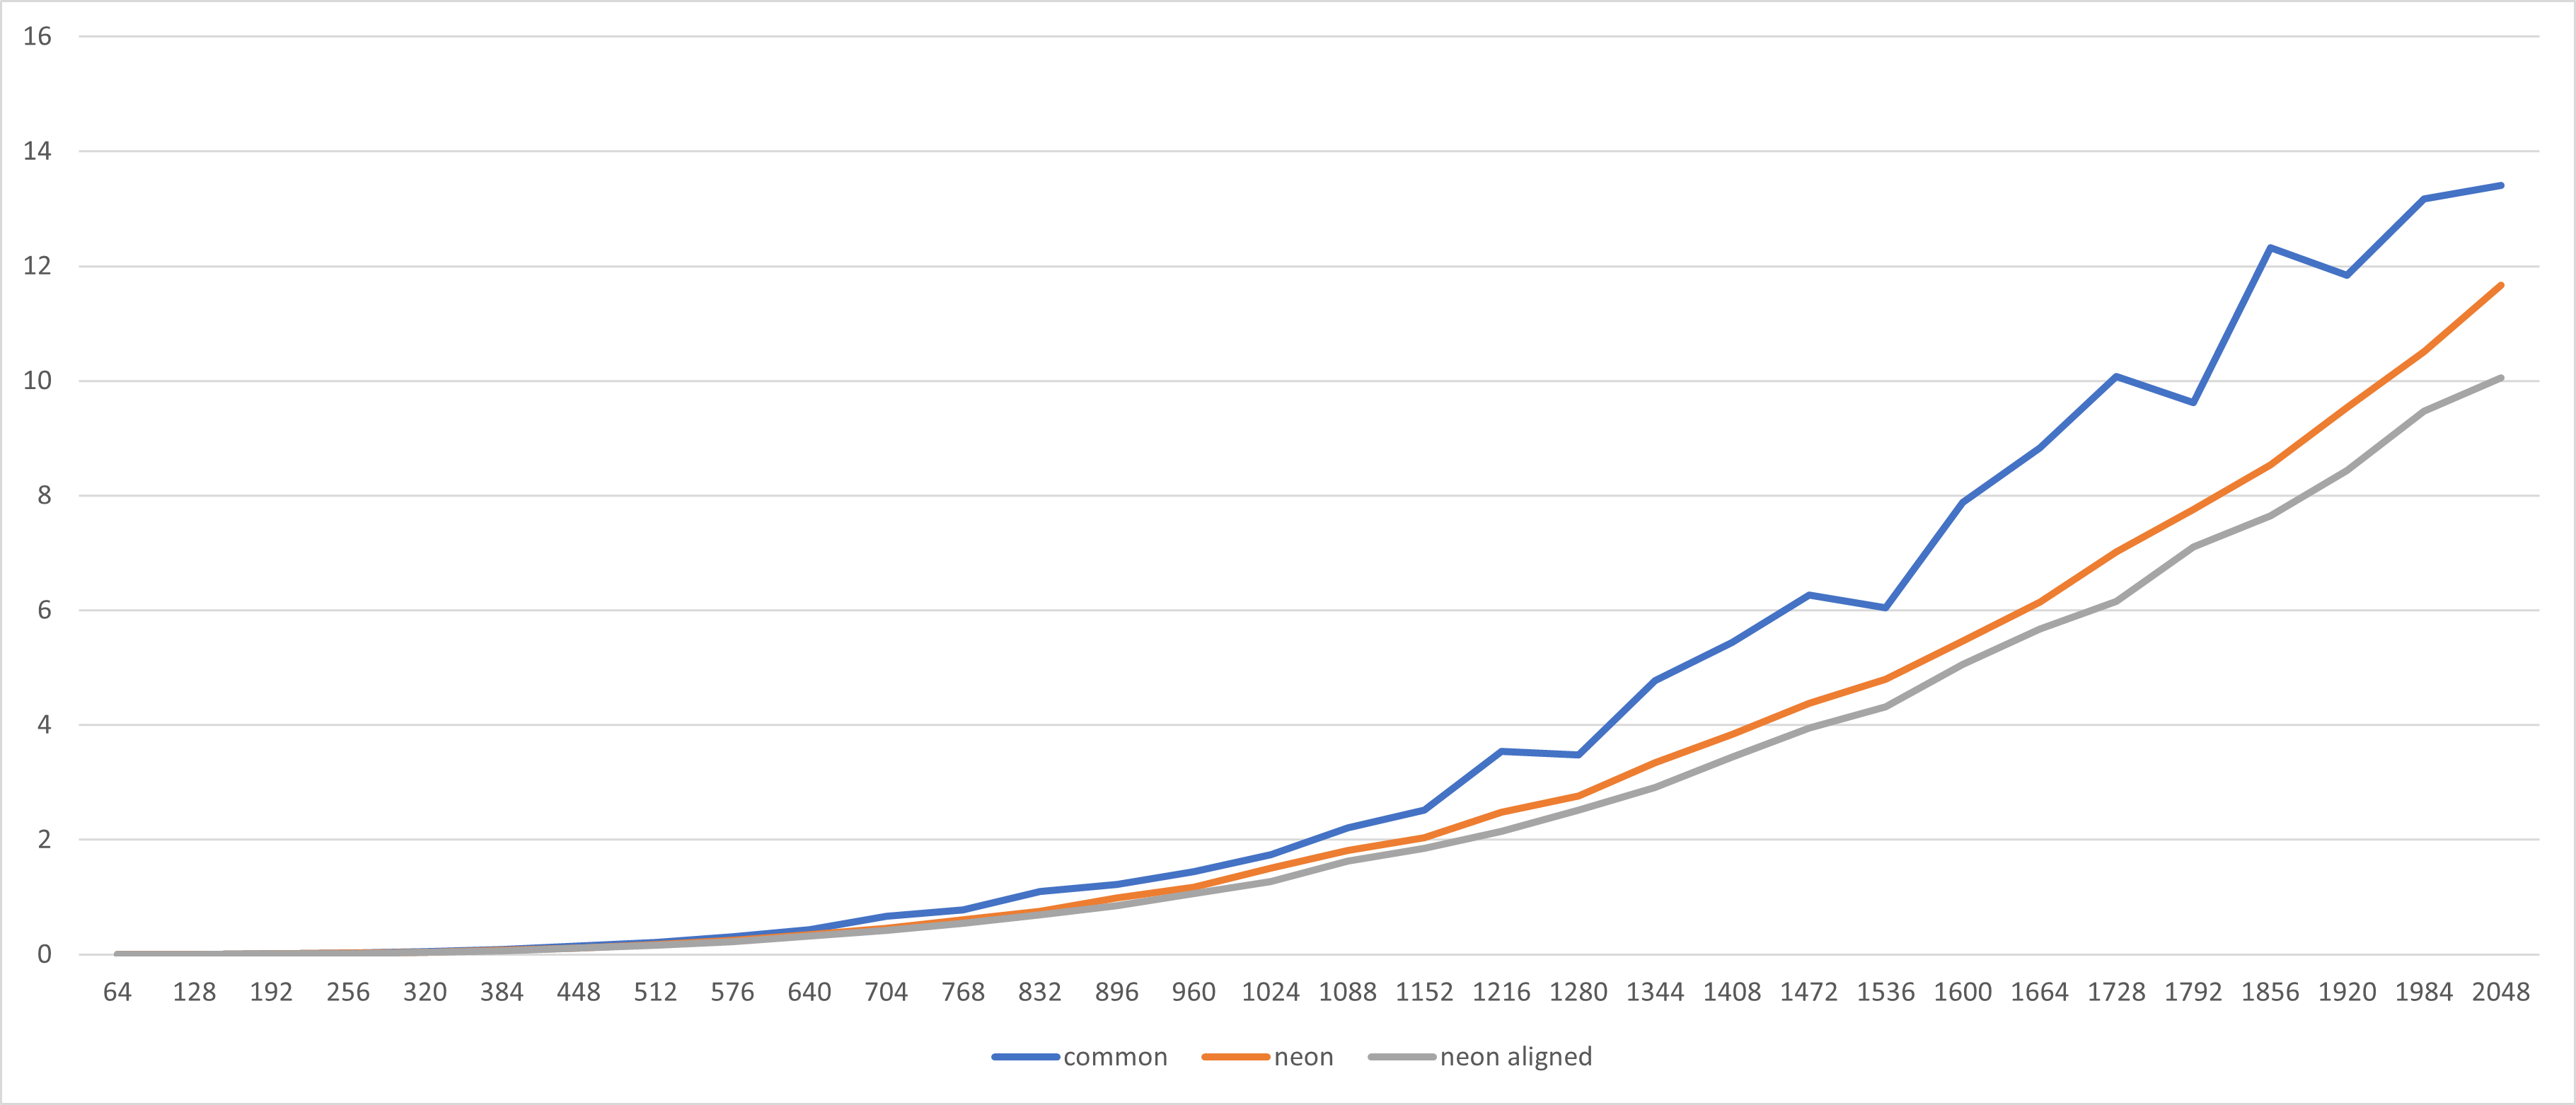
\includegraphics[width=6.2in]{fig/arm_gauss_timing.png}
    \caption{ARM平台下普通高斯消去算法 运行时间-输入数据规模(矩阵元素数量)}
    \label{fig:arm_gauss_timing}
\end{figure}

\begin{figure}[H]
    \centering
    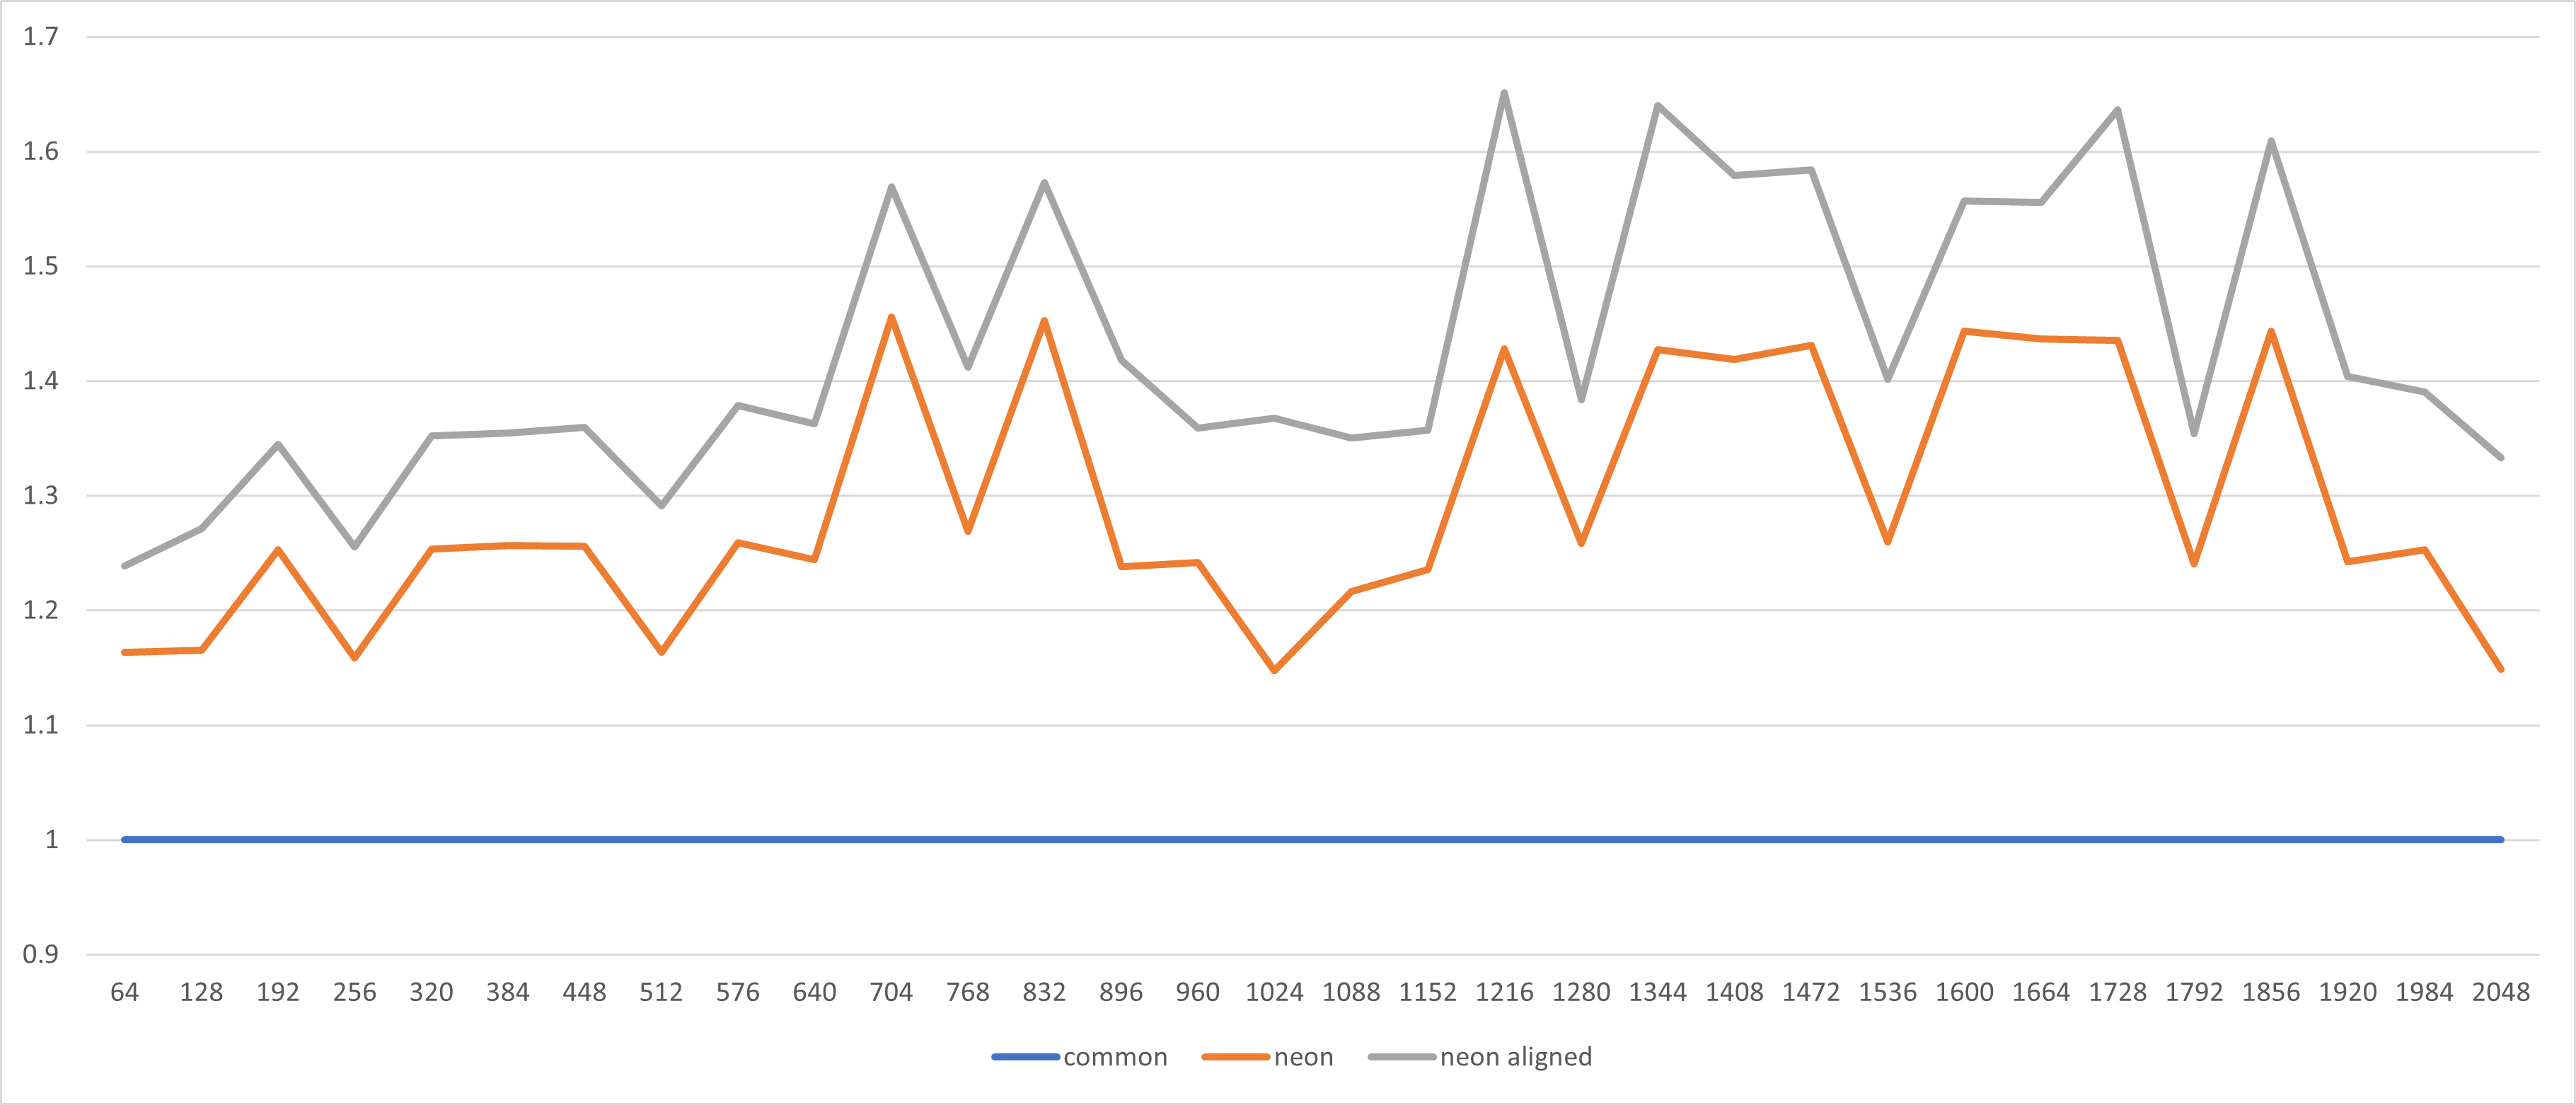
\includegraphics[width=6.2in]{fig/arm_gauss.png}
    \caption{ARM平台下普通高斯消去算法 加速比-输入数据规模(矩阵行数)}
    \label{fig:arm_gauss}
\end{figure}

\newpage
X86平台下普通高斯消去算法的运行时间与加速比随输入数据规模的变化如下图\ref{fig:x86_gauss_timing}和图\ref{fig:x86_gauss}所示:

\begin{figure}[H]
    \centering
    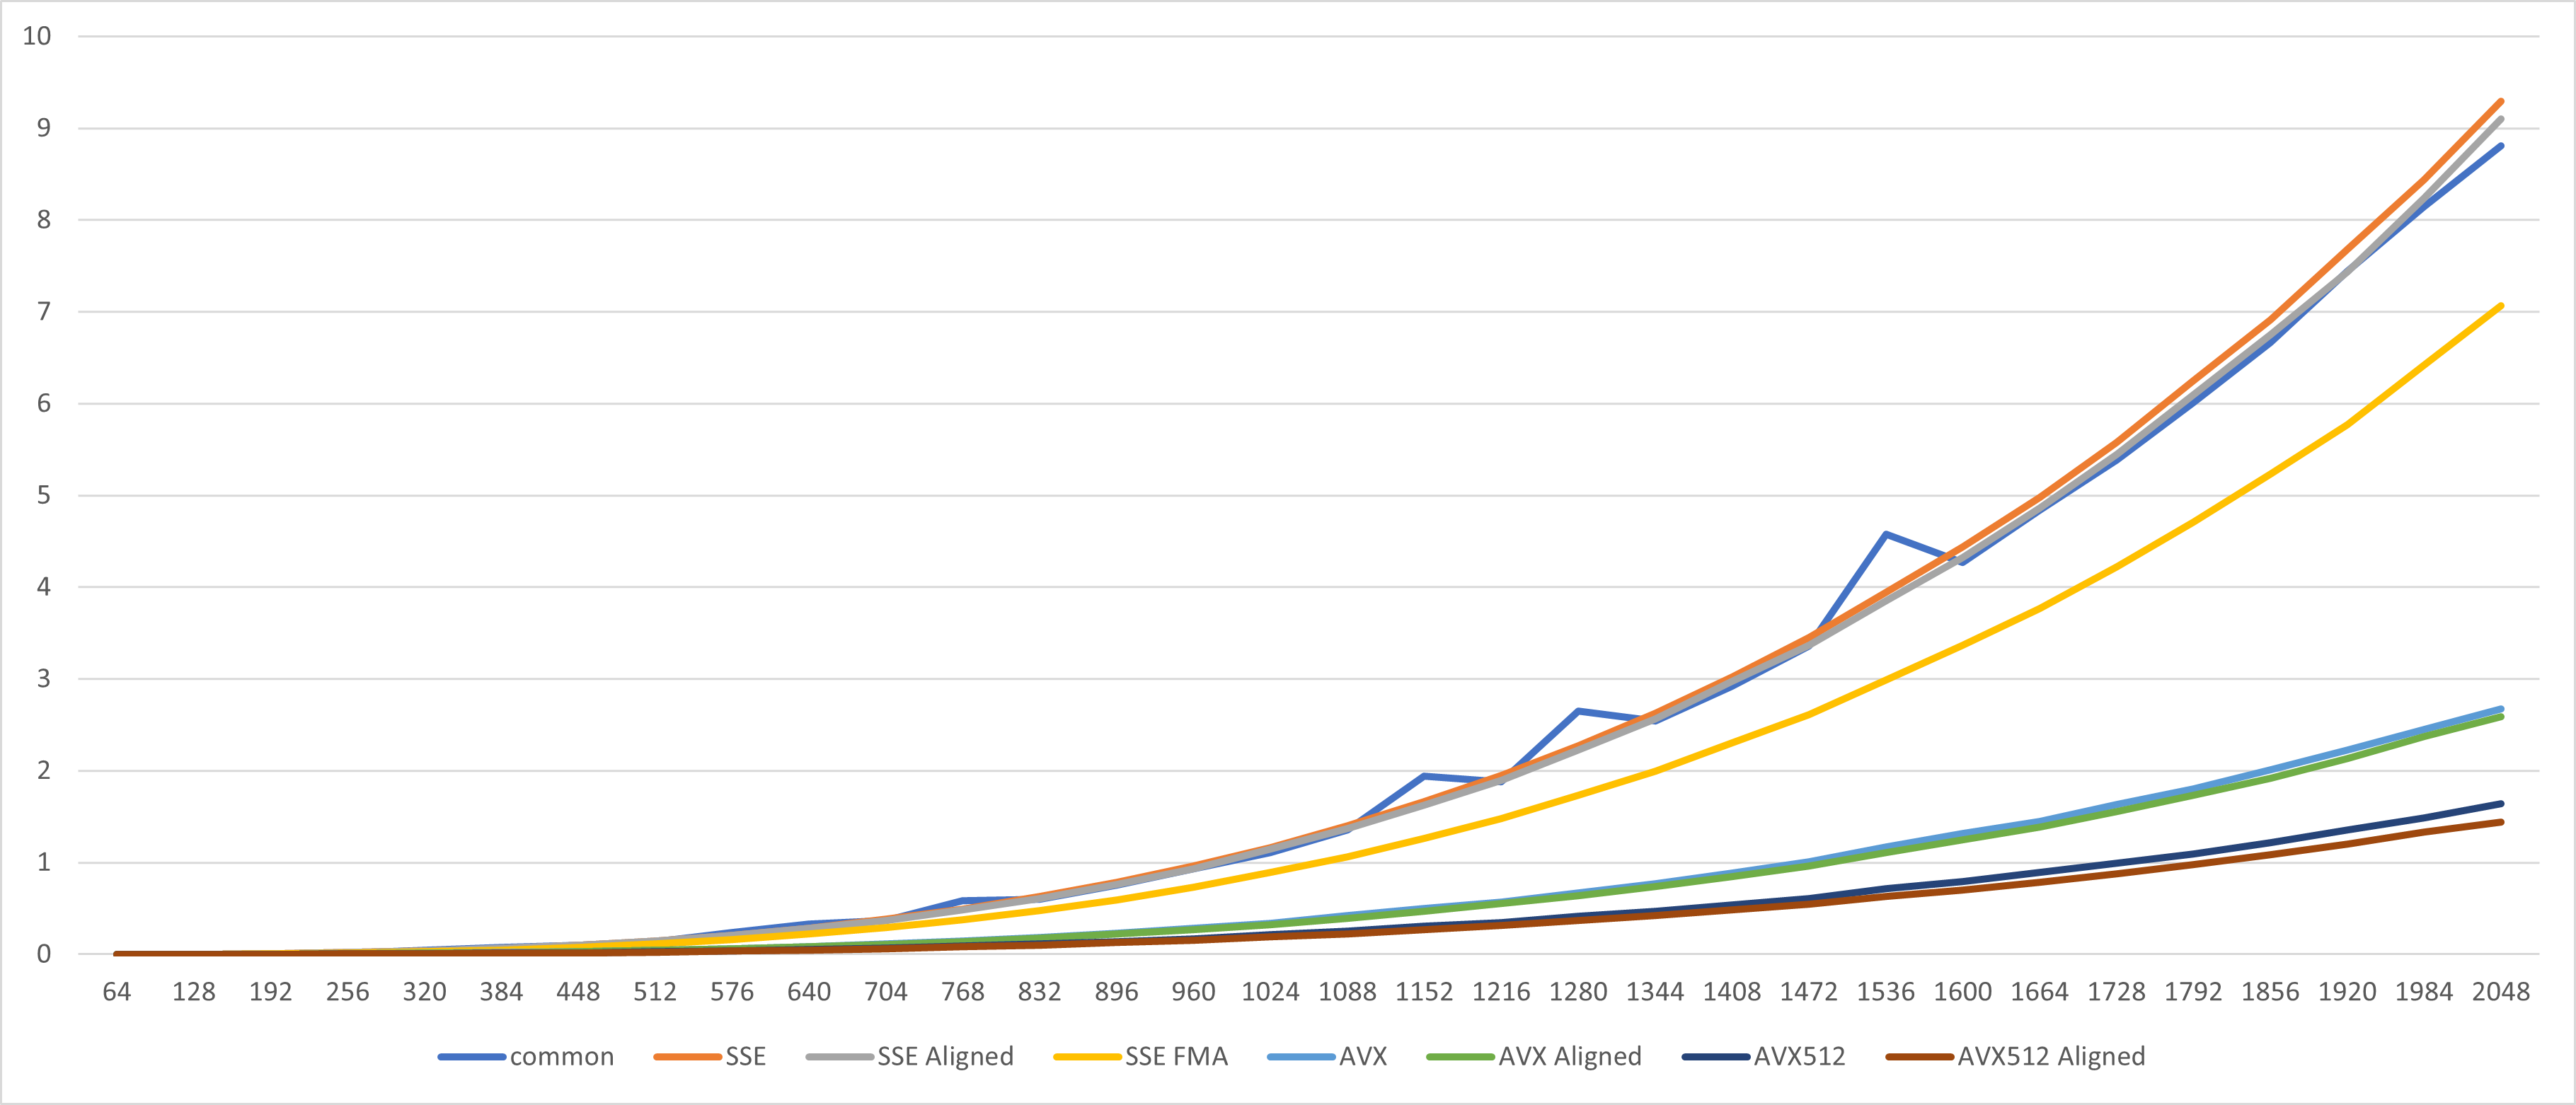
\includegraphics[width=6.2in]{fig/x86_gauss_timing.png}
    \caption{X86平台下普通高斯消去算法 运行时间-输入数据规模(矩阵元素数量)}
    \label{fig:x86_gauss_timing}
\end{figure}

\begin{figure}[H]
    \centering
    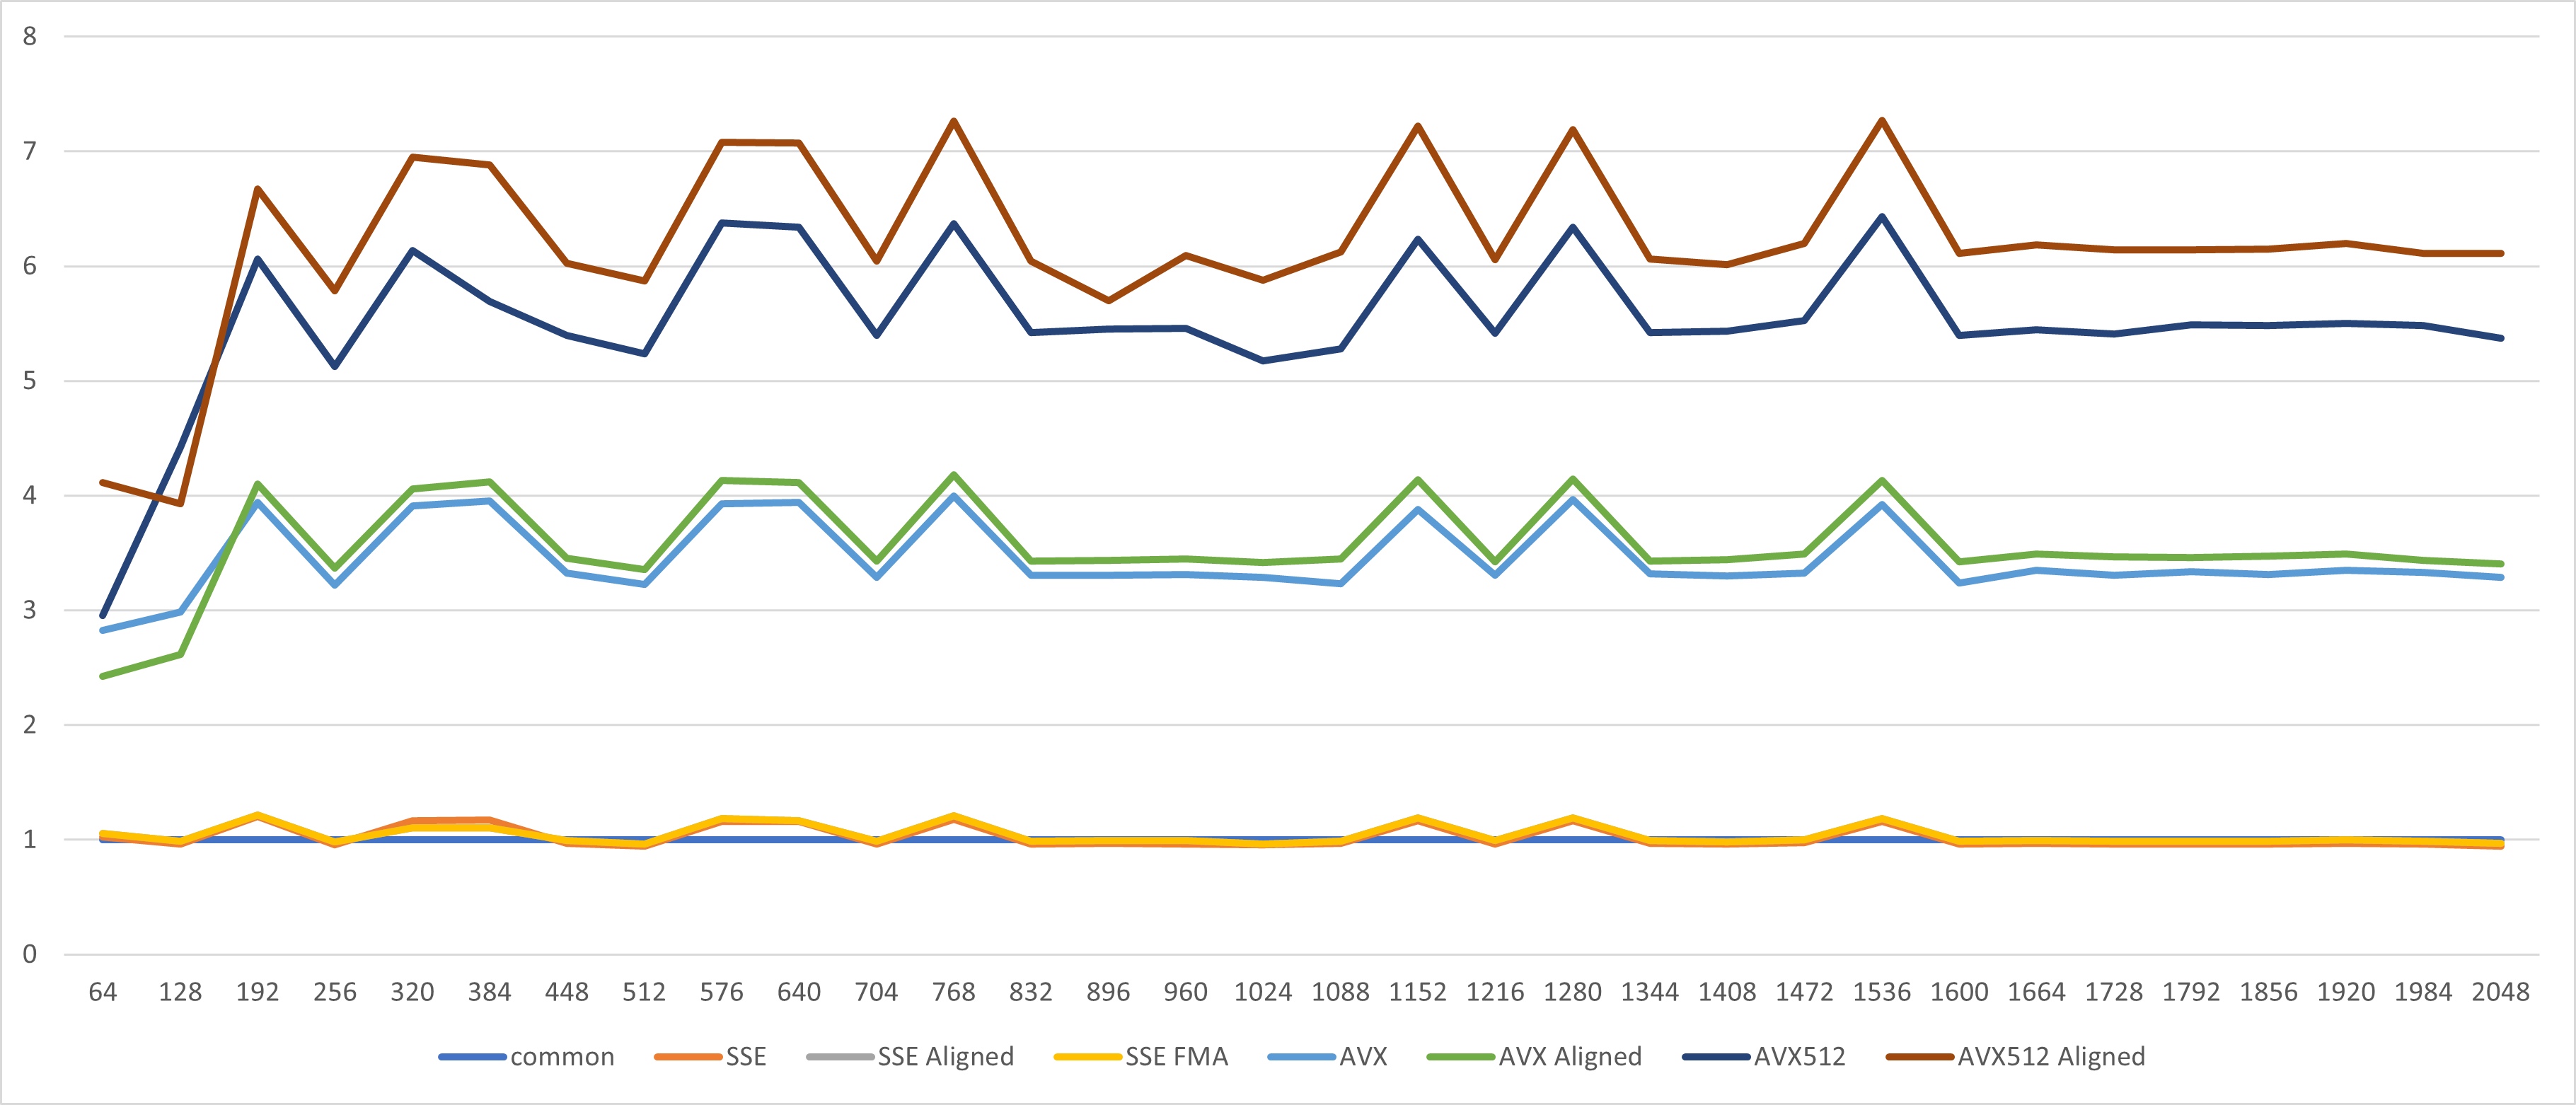
\includegraphics[width=6.2in]{fig/x86_gauss.png}
    \caption{X86平台下普通高斯消去算法 加速比-输入数据规模(矩阵行数)}
    \label{fig:x86_gauss}
\end{figure}

\subsection{消元子模式的高斯消去}

ARM平台下消元子模式高斯消去算法的运行时间与加速比随输入数据规模的变化如下表\ref{table:arm_groebner_timing}和图\ref{fig:arm_groebner}所示:

\begin{table}[H]
    \centering
    \begin{tabular}{|l|l|l|l|l|}
    \hline
        数据规模$\backslash$算法 & common & NEON & common Aligned & NEON Aligned \\ \hline
        3900 & 0.00001170 & 0.00000952 & 0.00001810 & 0.00001830 \\ \hline
        40386 & 0.00048108 & 0.00049586 & 0.00020015 & 0.00022082 \\ \hline
        125326 & 0.0009686 & 0.00079003 & 0.0004358 & 0.00048054 \\ \hline
        810822 & 0.0296091 & 0.025032 & 0.00594479 & 0.00580893 \\ \hline
        3965798 & 0.30704 & 0.188946 & 0.0510181 & 0.0353391 \\ \hline
        17900888 & 5.14359 & 3.78769 & 1.43977 & 0.945123 \\ \hline
        91633090 & 73.3229 & 48.1242 & 24.6904 & 14.6562 \\ \hline
    \end{tabular}
    \caption{ARM平台下特殊高斯消去算法 运行时间(单位:s)-输入数据规模(矩阵元素数量)}
    \label{table:arm_groebner_timing}
\end{table}

\begin{figure}[H]
    \centering
    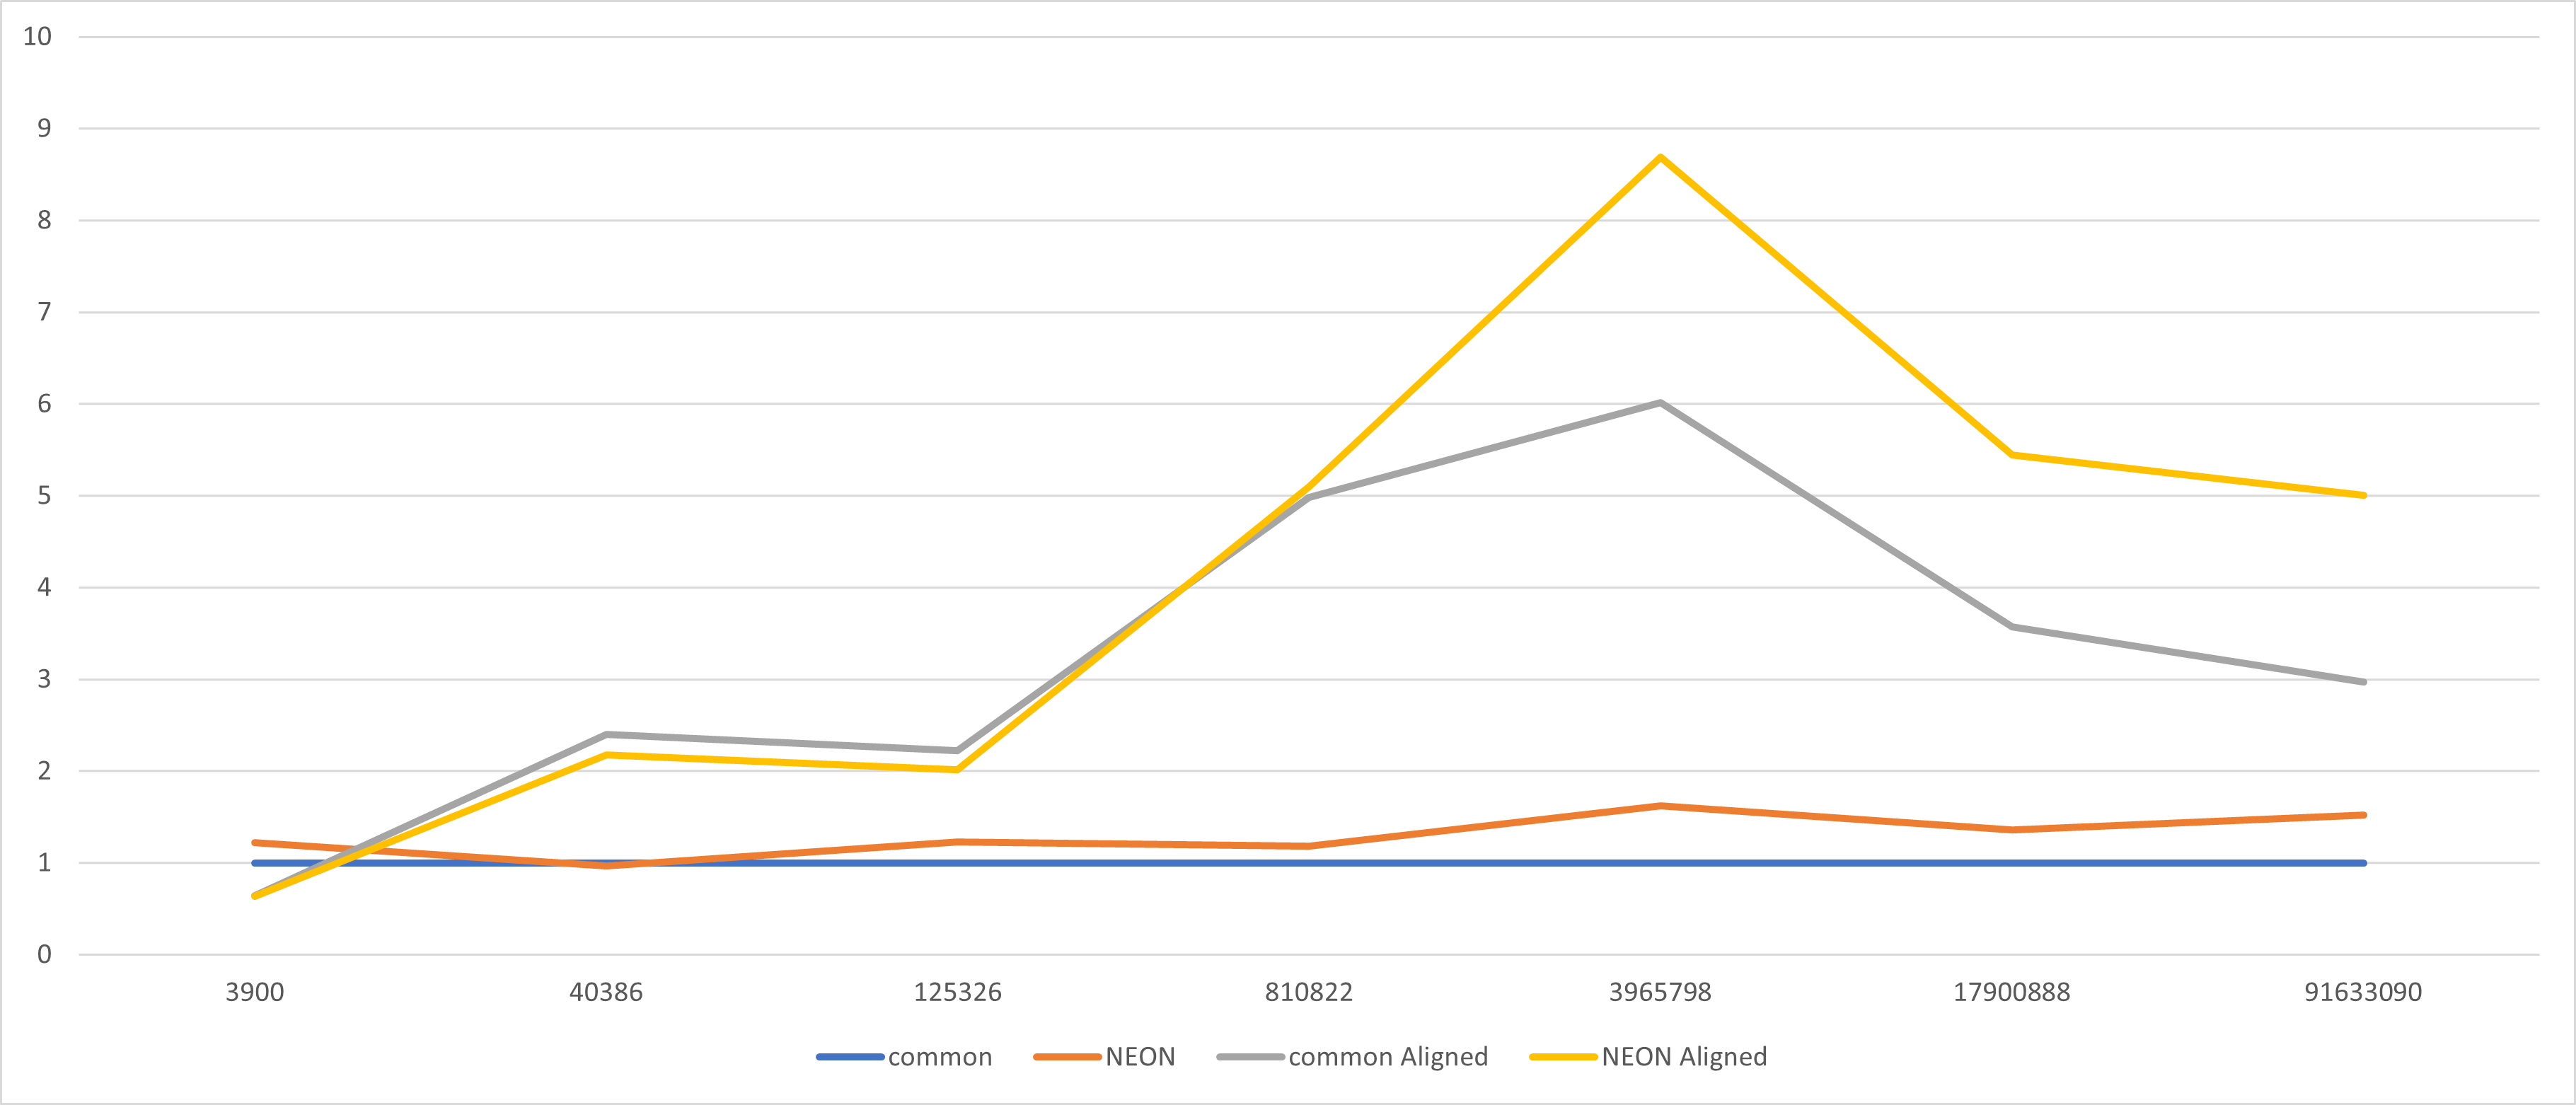
\includegraphics[width=6.2in]{fig/arm_groebner.png}
    \caption{ARM平台下特殊高斯消去算法 加速比-输入数据规模(矩阵元素数量)}
    \label{fig:arm_groebner}
\end{figure}

X86平台下消元子模式高斯消去算法的运行时间与加速比随输入数据规模的变化如下表\ref{table:x86_groebner_unaligned_timing}、表\ref{table:x86_groebner_aligned_timing}和图\ref{fig:x86_groebner}所示:

\begin{table}[H]
    \centering
    \begin{tabular}{|l|l|l|l|l|}
    \hline
        数据规模$\backslash$算法 & common & sse & avx & avx512 \\ \hline
        3900 & 0.000011 & 0.000007 & 0.000007 & 0.000007 \\ \hline
        40386 & 0.00040847 & 0.000377996 & 0.000392432 & 0.000448707 \\ \hline
        125326 & 0.000847442 & 0.000738246 & 0.000511157 & 0.000510796 \\ \hline
        810822 & 0.0264889 & 0.020673 & 0.015211 & 0.019706 \\ \hline
        3965798 & 0.205045 & 0.157969 & 0.0717809 & 0.0773024 \\ \hline
        17900888 & 3.53027 & 2.85676 & 1.29475 & 1.07147 \\ \hline
        91633090 & 46.0136 & 36.0756 & 14.8857 & 11.9147 \\ \hline
    \end{tabular}
    \caption{X86平台下特殊高斯消去不对齐算法 运行时间(单位:s)-输入数据规模(矩阵元素数量)}
    \label{table:x86_groebner_unaligned_timing}
\end{table}

\begin{table}[!ht]
    \centering
    \begin{tabular}{|l|l|l|l|l|}
    \hline
        数据规模$\backslash$算法 & common & sse & avx & avx512 \\ \hline
        3900 & 0.000017 & 0.000018 & 0.000013 & 0.000013 \\ \hline
        40386 & 0.000204125 & 0.000168772 & 0.000169869 & 0.000215989 \\ \hline
        125326 & 0.000384611 & 0.000369623 & 0.000382977 & 0.00039918 \\ \hline
        810822 & 0.00515151 & 0.00510496 & 0.00431197 & 0.00495711 \\ \hline
        3965798 & 0.0459342 & 0.0246126 & 0.0185454 & 0.0193652 \\ \hline
        17900888 & 1.14343 & 0.594648 & 0.397932 & 0.315436 \\ \hline
        91633090 & 16.3684 & 8.23317 & 5.05761 & 3.83209 \\ \hline
    \end{tabular}
    \caption{X86平台下特殊高斯消去对齐算法 运行时间(单位:s)-输入数据规模(矩阵元素数量)}
    \label{table:x86_groebner_aligned_timing}
\end{table}

\begin{figure}[H]
    \centering
    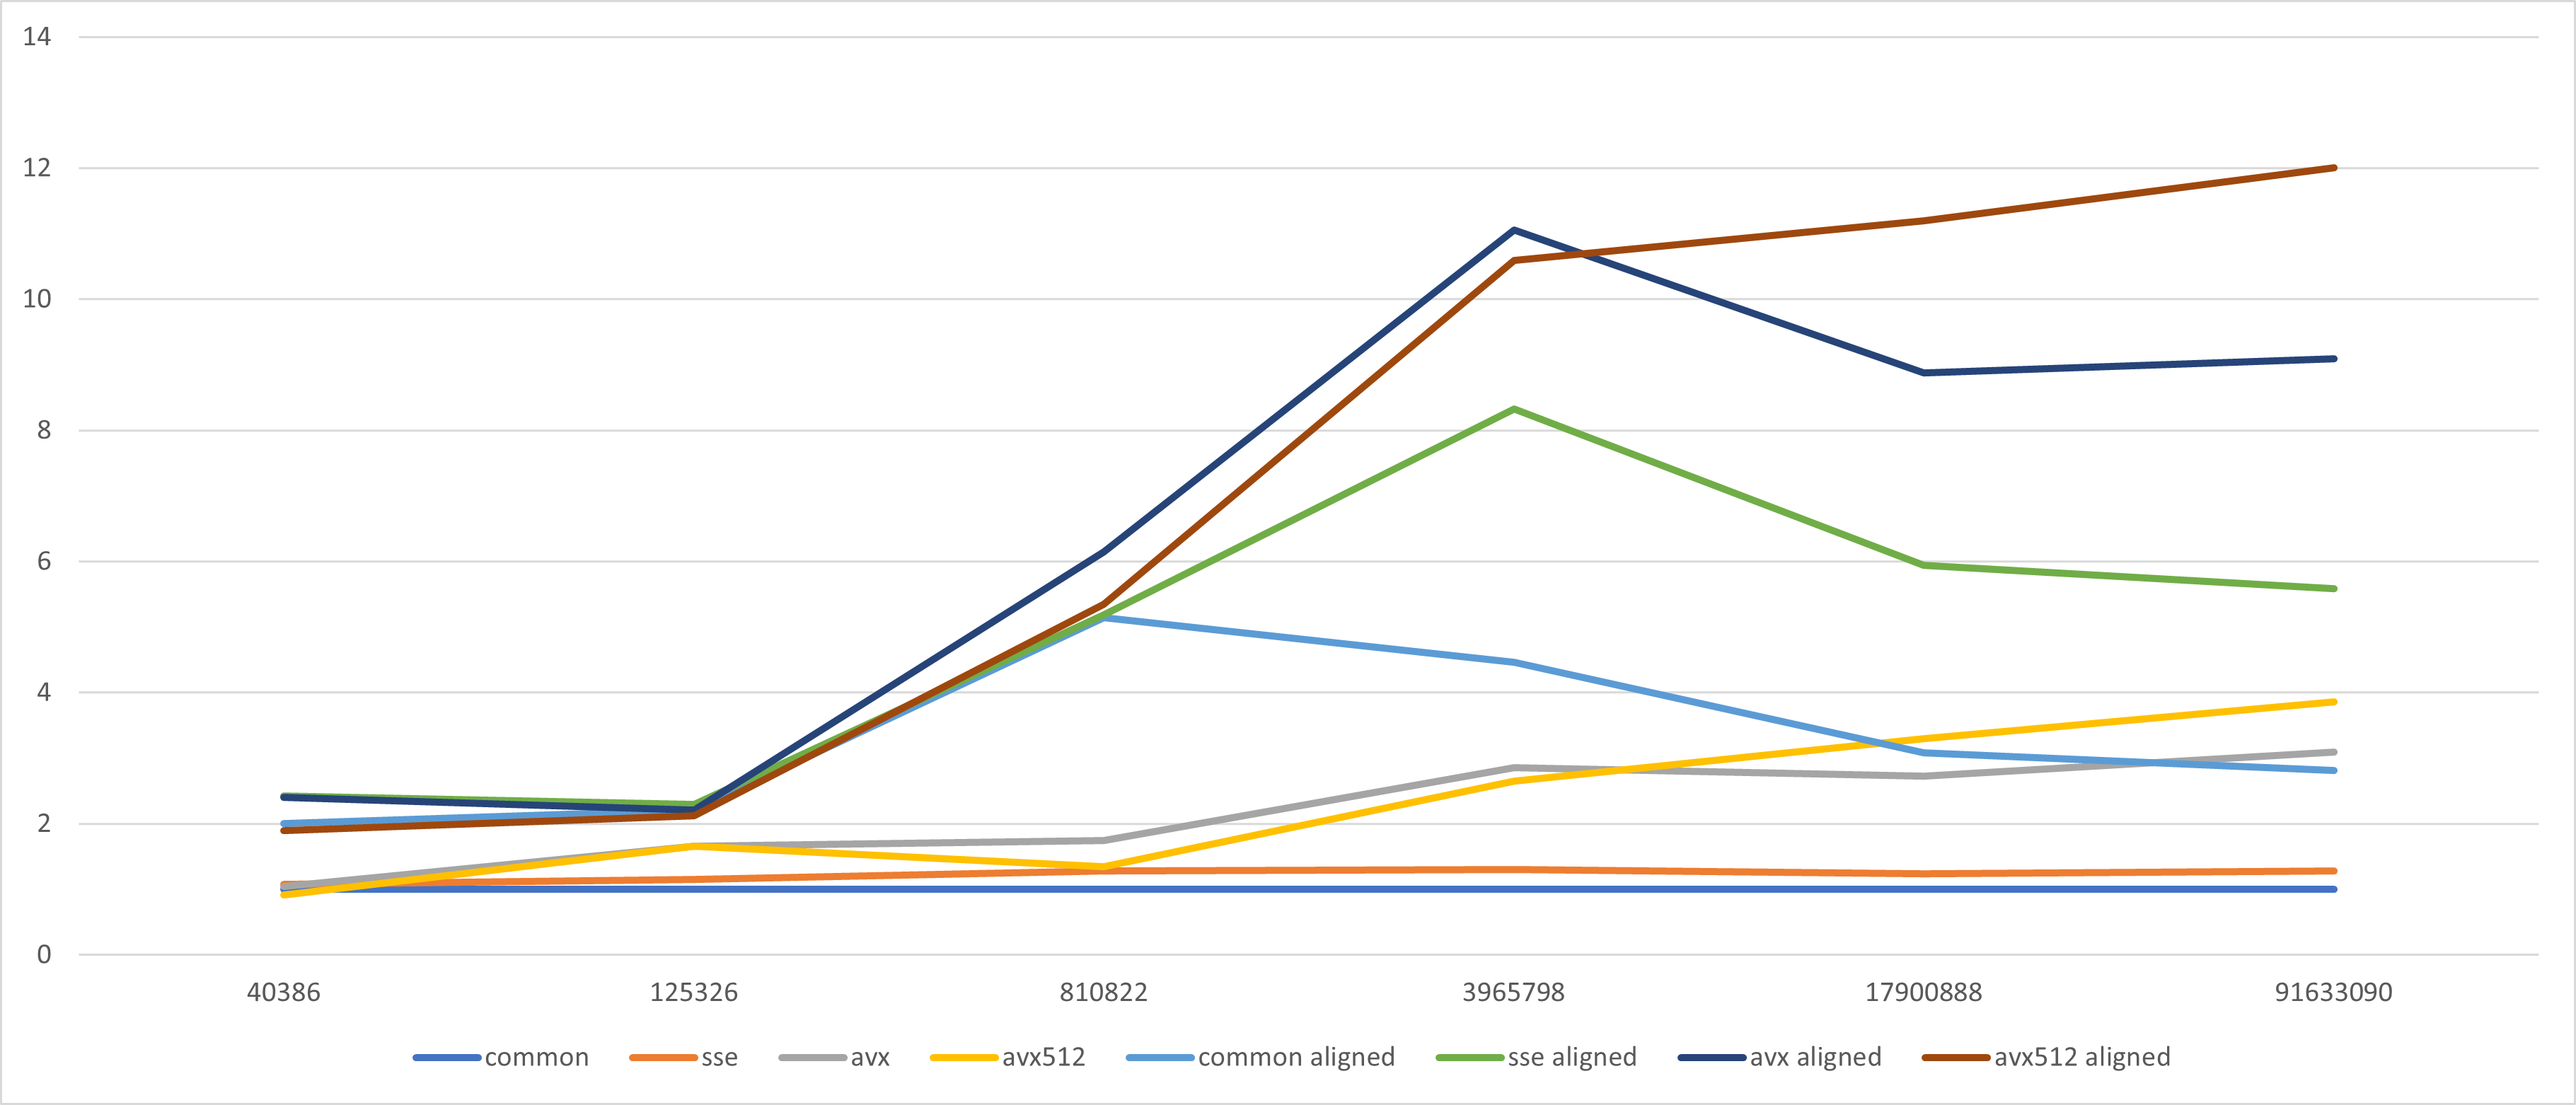
\includegraphics[width=6.2in]{fig/x86_groebner.png}
    \caption{X86平台下特殊高斯消去算法 加速比-输入数据规模(矩阵元素数量)}
    \label{fig:x86_groebner}
\end{figure}

\section{结果分析}
\subsection{不同SIMD指令集对比}

不难注意到,无论是在普通高斯消去(图\ref{fig:arm_gauss}和图\ref{fig:x86_gauss_timing})中,还是在消元子模式的高斯消去(图\ref{fig:arm_groebner}和图\ref{fig:x86_groebner})中,当数据规模达到一定水平后,寄存器位数越高的SIMD指令集,其加速比也越高。这是因为寄存器位数决定了一次运算可以处理数据的的数量,实验中使用的数据类型为unsigned int,AVX512寄存器位数为512,那么一次就可以处理16个数据,而128位的SSE和NEON就只能处理4个数据。

此外,SIMD运算中大量的Load/Store也导致了一定的性能损失,在一次Load/Store只能处理四个数据的SSE下更加降低了加速比。ARM平台上的perf事件计数表明,对齐的NEON加速特殊高斯消去算法的35\%的cycles都耗费在了vst1q函数上,这或许能解释为何NEON/SSE加速算法的运行时间有时甚至长于普通算法。

\subsection{数据对齐及Cache性能分析}

对于特殊高斯消去算法,在ARM平台和X86平台上,我们不难发现,即使只是简单的将矩阵的定义从$mat\_t ele\_tmp[COL][COL / mat\_L + 1];$改为$mat\_t ele\_tmp[COL][(COL / mat\_L + 1) / 16 * 16 + 16] \_\_attribute\_\_((aligned(64))) = {0};$也就是将二维数组的列数定义为16的整倍数,就可以给未使用SIMD的平凡算法带来最高5倍的加速比。

perf性能测量后发现,对于未使用SIMD的平凡算法,修改前后cache-misses事件的估计数量从39957488降低到了15547456,降幅达61.1\%;branch-misses事件的估计数量从16854480降低到5541842,降幅达67.12\%。

作者猜测,列数为16整倍数的二维数组可以更“整齐”的存放进Cache和内存中,而Cache和内存都是按字节块读取的,“整齐”的存放方式可以降低读取次数、提升性能。对齐的数据也能防止造成Cache的伪共享现象,进而充分利用CPU的超标量设计来提升性能。

此外,当需要在一个形如$arr[M][N]$二维数组中寻址元素$arr[i][j]$时,需要进行$i*N+j$这样的操作,而如果N是2的幂,经过编译器的优化,可以更快的运行乘法,这样也就加速了寻址的过程。

而如果对于SIMD加速算法,对齐的数据更可以减少Load/Store的次数,带来更高的性能。

\subsection{融合乘加所带来的性能影响}

如图\ref{fig:x86_gauss_timing}和图\ref{fig:x86_gauss}所示,SSE加速在使用融合乘加的情况下有较明显的性能提升,查阅英特尔的Intrinsics Guide\cite{intelintrinsicsguide}得知,乘法指令\_mm\_mul\_ps,减法指令\_mm\_sub\_ps,和融合乘减\_mm\_fnmadd\_ps指令延迟均为4个周期,CPI均为5,这样一来,使用融合乘加运算便可以在这一项上节约一半的时间,带来巨大的性能优势。

\newpage
\bibliographystyle{plain}
\bibliography{reference.bib} 

\end{document}